\documentclass[11pt]{ctexart}

\usepackage{multicol}
%\usepackage{mwe}
\usepackage{subfigure}
\usepackage{mathtools}
\usepackage{graphicx}
\usepackage{amsmath}
\usepackage{mathrsfs}
\usepackage[top=0.5in,bottom=1in,left=1in,right=1in]{geometry}
\usepackage{pdflscape}
\usepackage{times}
\usepackage{bm}
%\usepackage{setspace}
\usepackage{color}
\usepackage{caption}
\usepackage{amsmath}
\usepackage{amssymb}
\usepackage{CJK}
%\usepackage[final]{pdfpages}
\usepackage{listings}
\usepackage{textcomp}
\usepackage{xcolor}
\usepackage{algorithm2e}
\usepackage{float}
\usepackage{algorithmicx}
\usepackage{algpseudocode}
\usepackage{hyperref}

\hypersetup{hidelinks,
	colorlinks=true,
	allcolors=black,
	pdfstartview=Fit,
	breaklinks=true}

\pagestyle{plain}




\begin{document}

\title{第五周实习报告20220401}
\author{宋欣源}
\date{\today}

\maketitle % need full-width title

\CTEXsetup[format={\Large\bfseries}]{section}

\section{第一,综述}

首先,对任务进行了重新理解。

输入:raw5数据集,按照传统的时间序列增强办法,扩充为1-19个数据集,分别代表不同时间的股票数据,其中1-14为训练集,15,17,18,19为测试集,100为验证集。raw5数据集是(batchsize,490,3)的数据,对应每一天的batch,向前滑动10天,每天49根bar,3是3个特征,对应close,volume,turnover。

输出:y\_train和y\_eval数据集,代表日频close数据(不一定是close或vwap,反正是个抽象价格),

目的:利用前10日日内5min数据预测下一日的日频close数据。

可能做好的方向:

\begin{itemize}
  \item [1)]
  第一,既然是时间序列预测,能做的就是在之前的490根bar上进行cnn2d,cnn1d,rnn的使用,生成时间序列,然后再利用时间序列生成截面观点。之前做的工作依然可用,可以继续深挖。之前的工作主要内容是利用之前的490根bar模拟时间序列过程,生成下一根bar的截面价格数据。已经弄出了很复杂的模型。最后的结果,最高IC达到0.7,pnl达到2.4。如下图所示:
  
    \begin{figure}[htbp]
    \begin{center}
    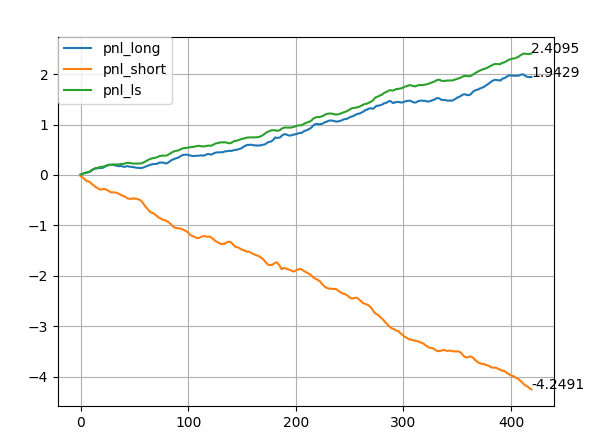
\includegraphics[width=0.8\textwidth]{2.4.PNG}
    \end{center}
    \caption{best pnl figure}
    \label{FIG.1}
    \end{figure}

    {\kaishu \small IC: 0.073, pnl:2.42}
  \item [2)]
  既然是日频价格数据,和根bar还不太一样。这个抽象价格如果是open,那就是上面的做法,可以继续深入。经过实验看来应该不是。因为从cnn2d,cnn1d,rnn三个角度都已经得出了非常相似的输出结果 了,说明以上三个办法,在可容忍的信噪比范围内,都已经很好的模拟出100bar的价格序列了,但是最后只能达到2.4,说明这个做法并非最终做法。最后的labels是下一日的统计数据,因此还应包含日频率的统计信息。
  \item [3)]
  从挖因子的角度讲,下一日的数据预测,一般是由日频预测和上一日日内分钟数据决定。(高频因子也是一样,下一根分钟bar数据,由之前的几十根分钟bar数据,和当前两根bar内的tick close数据决定)这样更符合统计观点,而且也确实涵盖了更多信息,因此之前的工作,主要从上一日和两日日内bar数据时间序列预测着手。下一步,应该用490bar数据,生成10day的日数据,利用day,half\_day数据对模拟的价格序列进行增强.事实证明两者相加果然效果提高很多。
  \item [4)]
  因此,从提高模型表达能力的角度出发,应该继续深化分钟时间序列研究,从原来的模型出发继续研究。从短期快速提高pnl的角度,将原来的研究应用于日频时间序列进行组合。从新的角度进行研究,不再研究时间序列,转而利用cnn2d,cnn1d直接研究截面,对界面进行模型研究是个新的方向。

\end{itemize}


\end{document} 